From the Mexico's National Institute of Geography and Statistics, INEGI, data from the 2010 census can be obtained. That year, 2351 Municipalities where censused and information is freely available at the institute web \href{http://www3.inegi.org.mx/sistemas/iter/entidad_indicador.aspx?ev=5}{page}.

As with the first example, the most significant digit of the population of each municipality was taken, and the frequency of repetition of each digit between 1 and 9 was compared with the prediction made by Benford's Law.

\begin{figure}[h!]
\centering
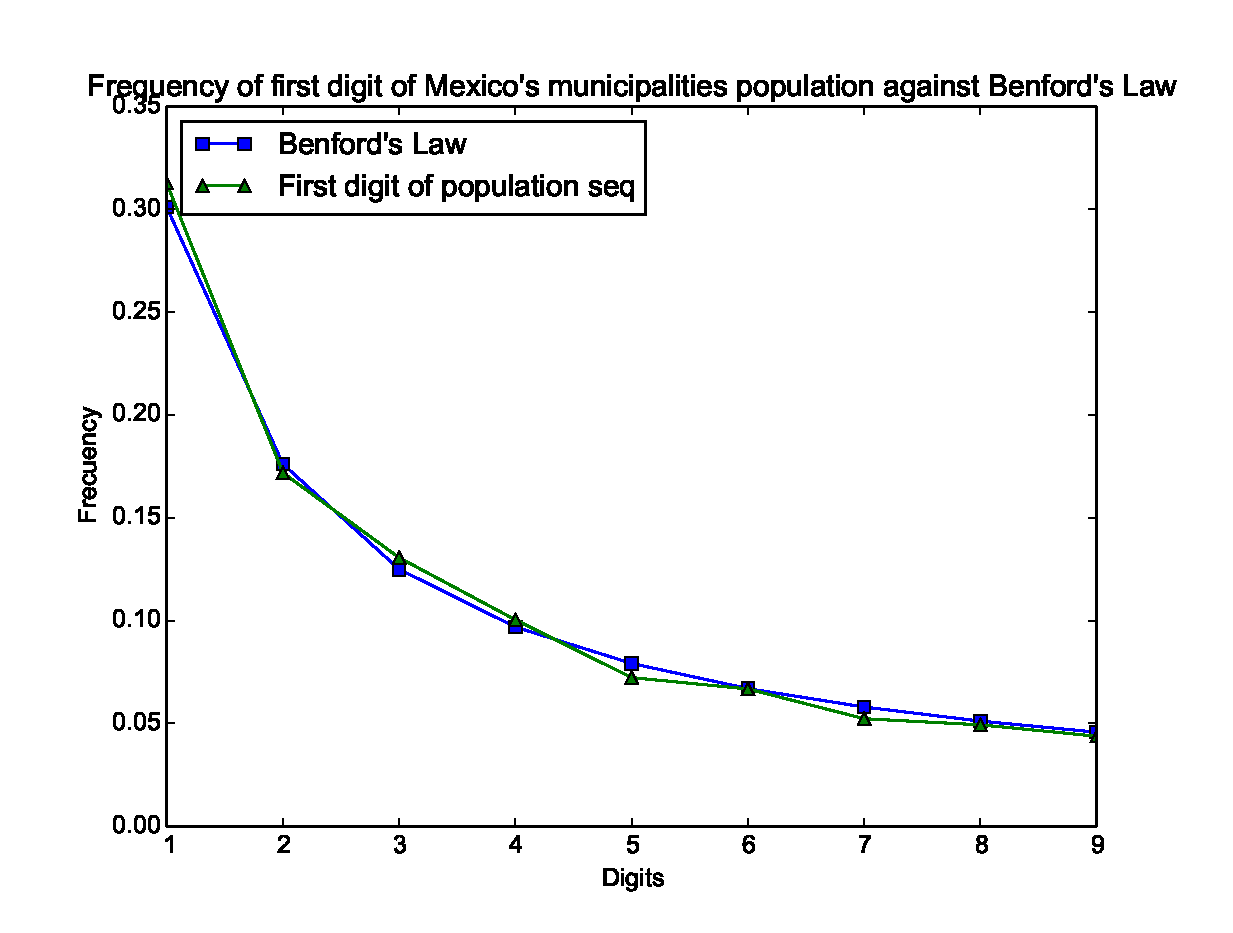
\includegraphics[scale=0.5]{imagenes/2-benford/benford_ex2}
\caption{Fibonacci Sequence against Benford's Law}
\end{figure}
